%%%%%%%%%%%%%%%%%%%%%%%%%%%%%%%%%%%%%%%%%%%%%%%%%%%%%%%%%%%%%%%%%%%%%%%%%%%%%%%
%%
%% Copyright © 2022 Tropic Square s.r.o. (https://tropicsquare.com/)
%%
%% This work is subject to the license terms of the LICENSE.txt file in the
%% root directory of this source tree.
%%
%% If a copy of the LICENSE file was not distributed with this work, you can
%% obtain one at (https://tropicsquare.com/license).
%%
%%%%%%%%%%%%%%%%%%%%%%%%%%%%%%%%%%%%%%%%%%%%%%%%%%%%%%%%%%%%%%%%%%%%%%%%%%%%%%%
%
% This is SPECT programmers manual
%
%%%%%%%%%%%%%%%%%%%%%%%%%%%%%%%%%%%%%%%%%%%%%%%%%%%%%%%%%%%%%%%%%%%%%%%%%%%%%%%

% Specify Tropic Square document class
\documentclass{tropic_design_spec}

\usepackage{listings}
\lstset{backgroundcolor=\color{lightgray}}

%%%%%%%%%%%%%%%%%%%%%%%%%%%%%%%%%%%%%%%%%%%%%%%%%%%%%%%%%%%%%%%%%%%%%%%%%%%%%%%
% Document properties and title page
%%%%%%%%%%%%%%%%%%%%%%%%%%%%%%%%%%%%%%%%%%%%%%%%%%%%%%%%%%%%%%%%%%%%%%%%%%%%%%%
\title{SPECT -- Programmer Guide}
\author{Vit Masek, Tropic Square}
\date{August 2023}

% Start of document
\begin{document}

% Parameters Needed by Design spec class (must be inside document)
% Set these parameters according to your project.
\def \projectname {SPECT}
\def \documentname {Programmer Guide ISAv0.2}
\def \versionnumber {0.1}

% Title page
\maketitle

\newcommand{\tspar}{\par\vspace{0.5cm}}
\newcommand{\tsspc}{\vspace{0.5cm}}
\newcommand{\tsblank}{\hspace*{0.5cm}}
\newcommand{\bi}[1]{\textbf{\textit{#1}}}

\newcommand{\tsnlind}{\newline\tsblank}

\newcommand{\tsif}{\textbf{\textit{if }}}
\newcommand{\tsthen}{\textbf{\textit{then: }}}
\newcommand{\tselse}{\newline\textbf{\textit{else: }}}

\def \G_RAR_DEPTH {5}


%%%%%%%%%%%%%%%%%%%%%%%%%%%%%%%%%%%%%%%%%%%%%%%%%%%%%%%%%%%%%%%%%%%%%%%%%%%%%%%
% Document revisions
%%%%%%%%%%%%%%%%%%%%%%%%%%%%%%%%%%%%%%%%%%%%%%%%%%%%%%%%%%%%%%%%%%%%%%%%%%%%%%%
\section*{Version history}

\begin{TropicRatioLongTable4Col}
    {0.1}            {0.2}                  {0.3}            {0.4}
    {Version Tag     & Date                 & Author          &    Description                    }
     0.1             & 7.8.2023             & Vit Masek       &    Initial version                \Ttlb
\end{TropicRatioLongTable4Col}

%%%%%%%%%%%%%%%%%%%%%%%%%%%%%%%%%%%%%%%%%%%%%%%%%%%%%%%%%%%%%%%%%%%%%%%%%%%%%%%
% External references
%%%%%%%%%%%%%%%%%%%%%%%%%%%%%%%%%%%%%%%%%%%%%%%%%%%%%%%%%%%%%%%%%%%%%%%%%%%%%%%

\newpage

\section*{Bibliography}

\begin{thebibliography}{9}

\bibitem{SHA512SPEC}
{FIPS 180-4}

\url{https://csrc.nist.gov/pubs/fips/180-4/upd1/final}

\bibitem{TROPIC01}
{TROPIC01 Repository}

\url{https://tropic-gitlab.corp.sldev.cz/internal/tropic01/tassic}

\bibitem{CRYPTOBLOCKS}
{ts-crypto-blocks}

\url{https://tropic-gitlab.corp.sldev.cz/internal/development-environment/ts-crypto-blocks}

\bibitem{SPECTFW}
{ts-spect-fw}

\url{https://tropic-gitlab.corp.sldev.cz/internal/sw-design/ts-spect-fw}

\bibitem{SCB}{
    Danger, Jean-Luc et al.
    “A synthesis of side-channel attacks on elliptic curve cryptography in smart-cards.”
    Journal of Cryptographic Engineering 3 (2013): 241 - 265.
}

\end{thebibliography}



%%%%%%%%%%%%%%%%%%%%%%%%%%%%%%%%%%%%%%%%%%%%%%%%%%%%%%%%%%%%%%%%%%%%%%%%%%%%%%%
% Table of contents
%%%%%%%%%%%%%%%%%%%%%%%%%%%%%%%%%%%%%%%%%%%%%%%%%%%%%%%%%%%%%%%%%%%%%%%%%%%%%%%
\pagebreak
\tableofcontents

%%%%%%%%%%%%%%%%%%%%%%%%%%%%%%%%%%%%%%%%%%%%%%%%%%%%%%%%%%%%%%%%%%%%%%%%%%%%%%%
%%%%%%%%%%%%%%%%%%%%%%%%%%%%%%%%%%%%%%%%%%%%%%%%%%%%%%%%%%%%%%%%%%%%%%%%%%%%%%%
% Document
%%%%%%%%%%%%%%%%%%%%%%%%%%%%%%%%%%%%%%%%%%%%%%%%%%%%%%%%%%%%%%%%%%%%%%%%%%%%%%%
%%%%%%%%%%%%%%%%%%%%%%%%%%%%%%%%%%%%%%%%%%%%%%%%%%%%%%%%%%%%%%%%%%%%%%%%%%%%%%%

%%%%%%%%%%%%%%%%%%%%%%%%%%%%%%%%%%%%%%%%%%%%%%%%%%%%%%%%%%%%%%%%%%%%%%%%%%%%%%%
% Glossary
%%%%%%%%%%%%%%%%%%%%%%%%%%%%%%%%%%%%%%%%%%%%%%%%%%%%%%%%%%%%%%%%%%%%%%%%%%%%%%%
\TsSection{Glossary}

\begin{itemize}
    \item{\textbf{CPU} - Central Processing Unit}
    \item{\textbf{ECC} - Elliptic Curve Cryptography}
    \item{\textbf{SPECT} - Secure Processor of Elliptic Curves for Tropic}
    \item{$P_{25519} = 2^{255} - 19$}
    \item{$P_{256} = 2^{256} - 2^{224} + 2^{192} + 2^{96} - 1$}
\end{itemize}

%%%%%%%%%%%%%%%%%%%%%%%%%%%%%%%%%%%%%%%%%%%%%%%%%%%%%%%%%%%%%%%%%%%%%%%%%%%%%%%
% Register field types
%%%%%%%%%%%%%%%%%%%%%%%%%%%%%%%%%%%%%%%%%%%%%%%%%%%%%%%%%%%%%%%%%%%%%%%%%%%%%%%
\TsSection{Register field types}

\TropicRegisterTypeList


%%%%%%%%%%%%%%%%%%%%%%%%%%%%%%%%%%%%%%%%%%%%%%%%%%%%%%%%%%%%%%%%%%%%%%%%%%%%%%%
% Introduction
%%%%%%%%%%%%%%%%%%%%%%%%%%%%%%%%%%%%%%%%%%%%%%%%%%%%%%%%%%%%%%%%%%%%%%%%%%%%%%%
\TsSection{Introduction}

This document provides a programmer's guide for SPECT. SPECT is a domain specific
processing unit targeted for calculations of Elliptic Curve Cryptography (ECC).
SPECT provides instructions for calculation with 256 bit numbers and modular
arithmetics. SPECT is useful to implement operations/algorithms such as:
\begin{itemize}
    \item{ECDSA -- Elliptic Curve Digital Signature Algorithm}
    \item{ECDH  -- Elliptic Curve Diffe-Hellman}
\end{itemize}

\begin{figure}[h!]
    \centering
    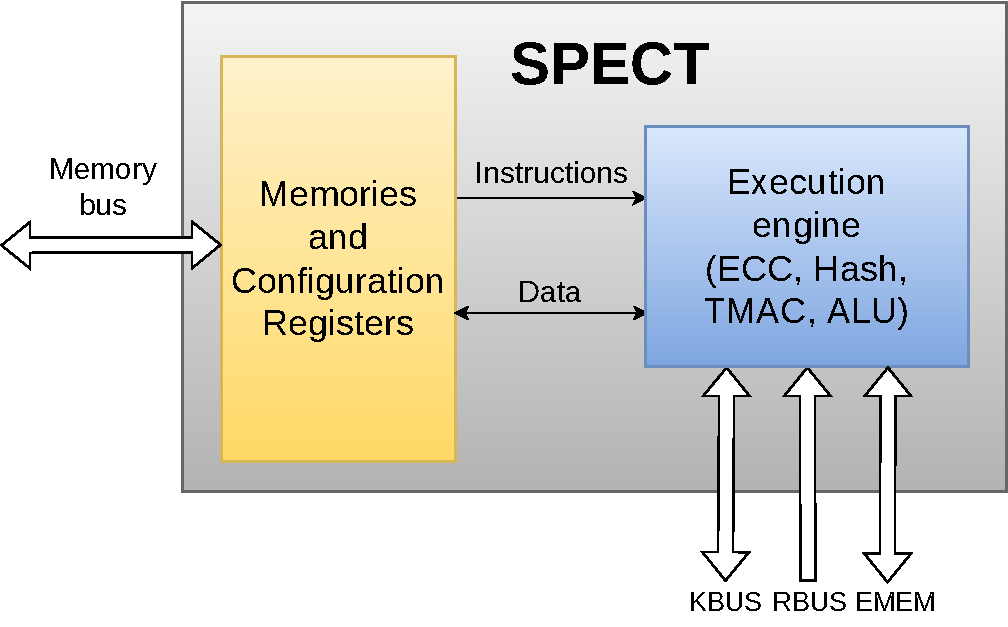
\includegraphics[width=\textwidth,height=\textheight,keepaspectratio]{%
        \detokenize{img/spect_pm_block_diagram.pdf}%
    }
    \caption{SPECT -- Block diagram}%
    \label{SPECTBK}%
\end{figure}

\TsSection{Programmer's model}

SPECT programmer's model consists of:
\begin{itemize}
    \item 32 x 256 bit general purpose registers (\textbf{R0} - \textbf{R31}).
    \item \textbf{PC} - Program counter.
    \item Zero (\textbf{Z}), Carry (\textbf{C}) and Error (\textbf{E}) flag.
    \item HW \textbf{RAR} (Return Address Register) stack for nested procedure calls.
    \item 2048 B read-write memory space in address range 0x0000 -- 0x07FC.
    \item 512 B write-only memory space in address range 0x1000 -- 0x11FC.
    \item 2048 B read-only memory space in address range 0x3000 -- 0x37FC.
    \item 144 B read-only memory space in address range 0x4000 -- 0x408C.
    \item 144 B read-only memory space in address range 0x4000 -- 0x408C.
    \item 50 B write-only memory space in address range 0x5000 -- 0x504C.
\end{itemize}

\TropicNote{
    SPECTs address space is 32 bit word organized. Load and store
    instructions works with 256 bit values and it always uses 8 consecutive words
    in the memory. E.g. 0x0020 - 0x003C.
}

\begin{figure}[h!]
    \centering
    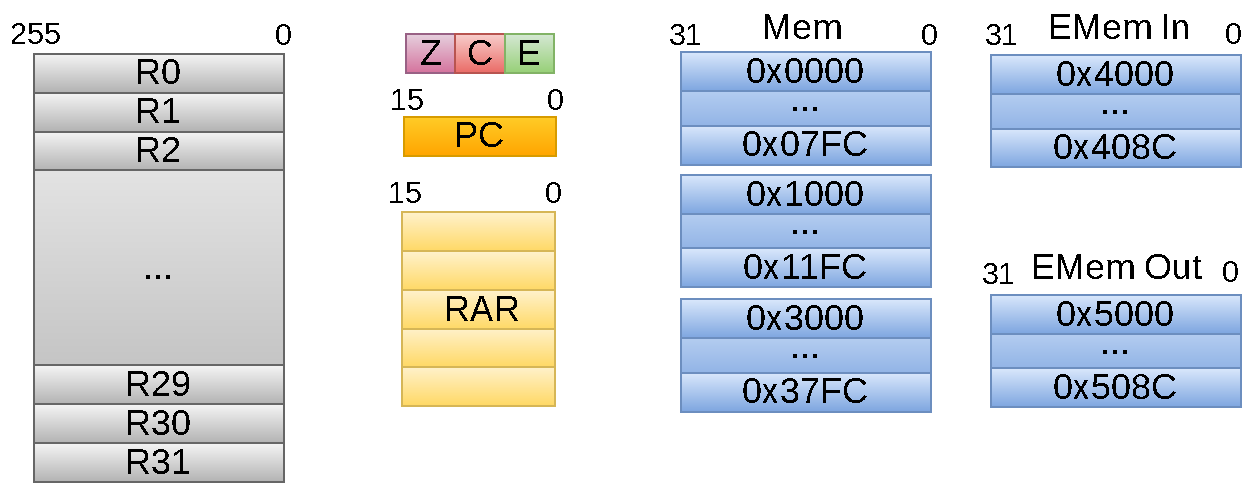
\includegraphics[width=.9\textwidth]{%
        \detokenize{img/spect_pm_gprs.pdf}%
    }
    \caption{SPECT -- Programmer model}%
    \label{SPECTBK}%
\end{figure}


\TsSubSection{Subroutine calls}

SPECT contains HW \textbf{RAR} stack, and it pushes return address from subroutine
to RAR stack each time when it executes CALL instruction. When SPECT executes
RET instruction, it pops value from RAR stack and updates \textbf{PC}. HW \textbf{RAR}
stack supports up to \G_RAR_DEPTH nested subroutine calls.

\TropicNote{
    Behavior of SPECT when number of nested subroutine calls is exceeded is undefined.
}

\TsSubSection{KBUS}

SPECT HW implements special 32 bit BUS interface (KBUS) to store and load cryptographic keys.
Particular key within the system is identified by following parameters:
\begin{itemize}
    \item Type -- Type of the key (ECC, SHPUB, STPRIV etc.). It specifies the location
                  of tke key in the system.
    \item Slot -- Particular key slot of the specified type. One slot can contain multiple related keys
                  (E.g. scalar and prefix in case of EdDSA).
    \item Offset -- Offset within the slot. Specifies position of the particular key.
\end{itemize}

SPECT ISA provides three instruction for KBUS -- LDK, STK, KBO. LDK is used to load keys, STK to store keys
and KBO for further control of the KBUS. Because SPECT operates with 256 bit values, both LDK and STK execute 8
consecutive KBUS transactions incrementing the offset.

For purpose of this document, notation KBUS_READ[type,slot,offset] indicates result of 8 consecutive
KBUS read transactions (increasing offset). Data from the first transaction are considered as LSBs,
data from the last transaction are considered as MSBs.

Further, notation KBUS_WRITE[key,type,slot,offset] indicates 8 consecutive KBUS write transactions (increasing offset)
with wdata = key. In first transaction, wdata = key[31:0]. In the last transaction, wdata = key[255:223].
KBUS_OP[type,slot,op] indicates one KBUS transaction of specific OP (e.g. "program slot").

Fore more information about KBUS, see TROPIC01 Functional Specification, Section 19 \cite{TROPIC01}.

\TsSubSection{RBUS}

SPECT HW implements special 32 bit interface for requesting random numbers from the external systems RNG.
SPECT ISA provides possibility to fetch 256 bit random number with GRV instruction.

\TsSubSection{Modular arithmetics}

SPECT provides instructions for finite field arithmetic such as
addition, subtraction and multiplication with 256 bit operands stored in general purpose
registers. SPECT supports fast multiplication in Ed25519 and P-256 curves finite fields 
via dedicated instructions -- MUL25519 and MUL256. Modular arithmetics with generic modulus
specified by value in \textbf{R31} is supported by instructions ADDP, SUBP, MULP. SPECT
also supports modular reduction of 512 bit number with REDP instruction.

When programming with modular instructions, one needs to be careful about input
operands of such instructions. Following conditions must be met:
\begin{itemize}
    \item op2 < $P_{25519}$ and op3 < $P_{25519}$ for MUL25519 instruction.
    \item op2 < $P_{256}$ and op3 < $P_{256}$ for MUL256 instruction.
    \item op2 < R31 and op3 < R31 for ADDP, SUBP instructions.
    \item R31 != 0 and R31 != 1 for ADDP, SUBP, MULP, REDP instructions.
\end{itemize}
if these conditions are not met when invoking such a instruction, result
of the instruction calculation is undefined (value in op1).

\TropicNote{
    Performance of MULP when \textbf{R31} = $P_{25519}$ / $P_{256}$ is lower
    than performance of MUL25519 / MUL256.
}

\TsSubSection{SHA512}

SPECT HW supports SHA512 Hash calculation as specified in \cite{SHA512SPEC}. SPECT can
calculate SHA512 hash from arbitrarily long data stream. When SPECT executes HASH_IT
instruction, it resets context in its execution engine to initialization
vector as specified in \cite{SHA512SPEC}. Each execution of HASH instruction
processes 1024 bit block, and executes next round of SHA512 calculation.

\TropicNote{
    SPECT HW does not add any padding of input data. It is responsibility of the firmware or
    external system to add such padding.
}

\TsSubSection{TMAC}

SPECT HW supports TMAC calculation as specified in TMAC documentation as part of ts-crypto-blocks repository \cite{CRYPTOBLOCKS}.
TMAC stands for Tropic Message Authentication Code. It is a custom MAC function inspired by KMAC function. It uses masked implementation
of KECCAK permutation with 400 bits internal state and rate of 18 bytes.

SPECT ISA provides four instructions for TMAC calculation.
\begin{itemize}
    \item TMAC_IT -- initialize underlying KECCAK core with 800 bits of mask and a guard.
    \item TMAC_IS -- initialize TMAC with initialization string as defined in TMAC specification.
    \item TMAC_UP -- updates internal state with another 18 bytes of data.
    \item TMAC_RD -- Squeeze 256 bits from the underlying KECCAK core as an output of the TMAC function.
\end{itemize}

\TsSubSection{Group Scalar Blinding}

SPECT HW supports scalar blinding by a random number as a side-channel counter-measure
with SCB instruction. It blinds the scalar $sc$ using group scalar randomization method
as defined in \cite{SCB} with 256 bit random number. The random number $rng$ shall be obtained in
advance by GRV instruction as described above. The group order $q$ shall be present in \textbf{R31}.

SCB performs this exact function: $$Blind(sc, rng, q) = q \times (rng | (2^{255} + 2^{223})) + sc$$

\TsSubSection{SPECT invocation}

SPECT firmware execution is invoked by external system that has access to its memory space via
memory bus as shown in following figure:

\begin{figure}[h!]
    \centering
    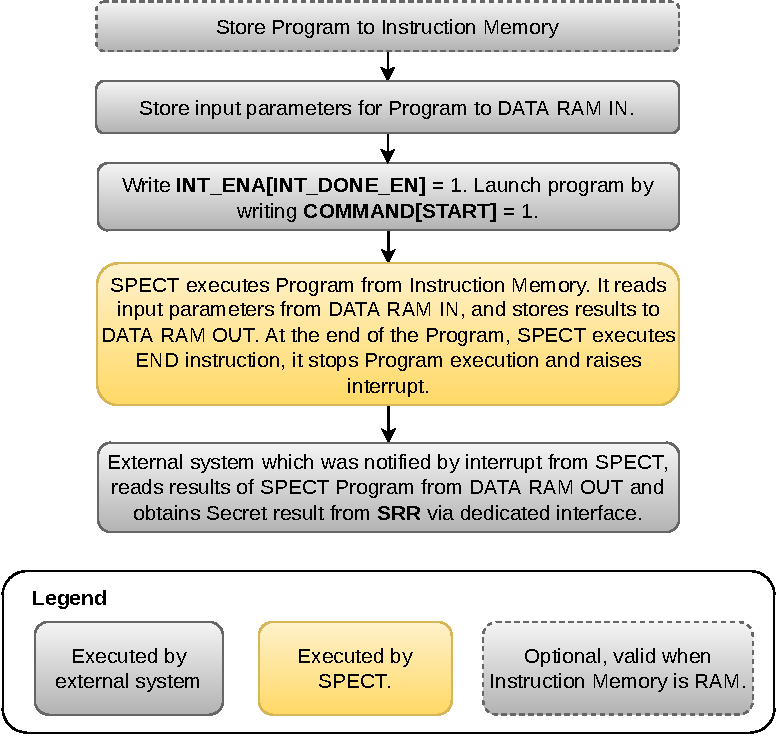
\includegraphics[width=.7\textwidth]{%
        \detokenize{img/spect_pm_invocation.pdf}%
    }
    \caption{SPECT -- Invocation}%
    \label{SPECTBK}%
\end{figure}

\TropicNote{
    Address of the first instruction executed by SPECT after
    \Register{COMMAND[START]} = 1 is written, is fixed and defined
    by a system that integrates SPECT.
}

\TsSubSection{Invalid instructions}

When SPECT attempts to execute invalid instruction, it aborts firmware execution
and sets \Register{STATUS[ERR]} = 1.

\TropicNote{
    Invalid instruction means invalid opcode or not matching parity bit in the instruction code. Unless
    a fault, usual cause of this is e.g. missing RET instruction in subroutine or END instruction at the
    end of the firmware execution.
}

\TsSubSection{Soft Reset}

SPECT can be reset by external system by writing \Register{COMMAND[SOFT_RESET]} = 1.
When SPECT is reset, it aborts any firmware execution and resets its internal state.

\TropicNote{
    Because GPRs are implemented as RAM, Soft Reset does not effect them in any way. GPRs can
    be cleared only by firmware.
}

\TsSubSection{Interrupts}

SPECT firmware execution can not be interrupted by an external event (other than
Soft Reset). SPECT itself can generate following interrupts for external system:
\begin{itemize}
    \item{Done -- Enabled when \Register{INT_ENA[INT_DONE_EN]} = 1.
                  Generated when SPECT firmware executes END instruction}
    \item{Error -- Enabled when \Register{INT_ENA[INT_DONE_EN]} = 1.
                   Generated when SPECT experience internal error (invalid instruction, bit-flip in SHA512 or TMAC core etc.)}
\end{itemize}


%%%%%%%%%%%%%%%%%%%%%%%%%%%%%%%%%%%%%%%%%%%%%%%%%%%%%%%%%%%%%%%%%%%%%%%%%%%%%%%
% Instruction set
%%%%%%%%%%%%%%%%%%%%%%%%%%%%%%%%%%%%%%%%%%%%%%%%%%%%%%%%%%%%%%%%%%%%%%%%%%%%%%%

\TsSection{Instruction set}

SPECT provides 4 types of instructions:
\begin{itemize}
    \item{\textbf{R} - Register}
    \item{\textbf{I} - Immediate}
    \item{\textbf{M} - Memory}
    \item{\textbf{J} - Jump}
\end{itemize}

\TsSubSection{Operand interpretation}

All operands are considered as 256 bits unsigned integers. Arithmetic instructions that work only with 32 bit
operands ignores the 224 MSBs of input and clears them in the result. Immediate logic instructions work only
with 12 LSBs, ignore the 224 MSBs of input, and pass the 244 MSBs of op2 to the result.

\TsSubSection{Instruction Format}

\definecolor{instgray}{RGB}{235, 235, 235}
    \begin{table}[h]
        \begin{center}
            \setlength{\tabcolsep}{4pt}
            \small
            \begin{tabular}{c c c c c c c c c c c c c c c c c c c c c c c c c c c c c c c c l}
            31 & 30 & 29 & 28 &
               &    & 25 & 24 &
               & 22 & 21 &    &
               &    & 17 & 16 &
            15 &    &    & 12 &
            11 &    &    &    &
            07 & 06 &    &    &
               &    &    & 00 & \\
            \hline
            \multicolumn{1}{|c|}{p} &
            \multicolumn{2}{c|}{\cellcolor{instgray}type} &
            \multicolumn{4}{c|}{\cellcolor{instgray}opcode} &
            \multicolumn{3}{c|}{\cellcolor{instgray}func} &
            \multicolumn{5}{c|}{\cellcolor{instgray}op1} &
            \multicolumn{5}{c|}{\cellcolor{instgray}op2} &
            \multicolumn{5}{c|}{\cellcolor{instgray}op3} &
            \multicolumn{7}{c|}{} &
            \textbf{R}\\
            \hline
            \\
            \hline
            \multicolumn{1}{|c|}{p} &
            \multicolumn{2}{c|}{\cellcolor{instgray}type} &
            \multicolumn{4}{c|}{\cellcolor{instgray}opcode} &
            \multicolumn{3}{c|}{\cellcolor{instgray}func} &
            \multicolumn{5}{c|}{\cellcolor{instgray}op1} &
            \multicolumn{5}{c|}{\cellcolor{instgray}op2} &
            \multicolumn{12}{c|}{\cellcolor{instgray}Immediate} &
            \textbf{I}\\
            \hline
            \\
            \hline
            \multicolumn{1}{|c|}{p} &
            \multicolumn{2}{c|}{\cellcolor{instgray}type} &
            \multicolumn{4}{c|}{\cellcolor{instgray}opcode} &
            \multicolumn{3}{c|}{\cellcolor{instgray}func} &
            \multicolumn{5}{c|}{\cellcolor{instgray}op1} &
            \multicolumn{1}{c|}{} &
            \multicolumn{16}{c|}{\cellcolor{instgray}Addr} &
            \textbf{M}\\
            \hline
            \\
            \hline
            \multicolumn{1}{|c|}{p} &
            \multicolumn{2}{c|}{\cellcolor{instgray}type} &
            \multicolumn{4}{c|}{\cellcolor{instgray}opcode} &
            \multicolumn{3}{c|}{\cellcolor{instgray}func} &
            \multicolumn{6}{c|}{} &
            \multicolumn{16}{c|}{\cellcolor{instgray}NewPC} &
            \textbf{J}\\
            \hline
            \end{tabular}
        \end{center}
        %\caption{Instruction Format}
    \end{table}

\TsSubSection{Symbols}

Following symbols are used in description of instructions:
\begin{itemize}
    \item{F -- Flags set by the instruction}
    \item{\#C -- Number of cycles the instruction takes to execute}
\end{itemize}


\begin{landscape}
\pagebreak
\TsSubSection{R instructions}
\begin{TropicRatioLongTable5Col}
    {0.25}                   {0.285}                              {0.4}                                         {0.03} {0.035}
    {Mnemonic               & Name                              & Semantics                                     & F     & \#C              }
      \TropicTableBreak{Arithmetic Instructions (32 bit)}                                                                       \Ttlb
      ADD op1,op2,op3       & 32 bit addition                   & op1 = op2 + op3                               & Z     & 11    \Ttlb
      SUB op1,op2,op3       & 32 bit subtraction                & op1 = op2 - op3                               & Z     & 11    \Ttlb
      CMP op2,op3           & 32 bit comparison                 & op2 - op3                                     & Z     & 9     \Ttlb

      \TropicTableBreak{Logic Instructions}                                                                                     \Ttlb
      AND op1,op2,op3       & Bitwise AND                       & op1 = op2 \& op3                              & Z     & 11    \Ttlb
      OR op1,op2,op3        & Bitwise OR                        & op1 = op2 | op3                               & Z     & 11    \Ttlb
      XOR op1,op2,op3       & Bitwise Exclusive OR              & op1 = op2 \textasciicircum\space op3          & Z     & 11    \Ttlb
      NOT op1,op2           & Bitwise NOT                       & op1 = \textasciitilde op2                     & Z     & 10    \Ttlb
      SBIT op1,op2,op3      & Set bit                           & op1 = op2 $\vee$ (0x1 $\ll$ op3[7:0])         &       & 11    \Ttlb
      CBIT op1,op2,op3      & Clear bit                         & op1 = op2 $\wedge$ $\sim$(0x1 $\ll$ op3[7:0]) &       & 11    \Ttlb


      \TropicTableBreak{Shift Instructions}                                                                                         \Ttlb
      LSL op1,op2           & Logic shift left                  & op1 = op2[254:0] || 0                 & C      & 10               \Ttlb
      LSR op1,op2           & Logic shift right                 & op1 = 0 || op2[255:1]                 & C      & 10               \Ttlb
      ROL op1,op2           & Rotating shift left               & op1 = op2[254:0] || op2[255]          & C      & 10               \Ttlb
      ROR op1,op2           & Rotating shift right              & op1 = op2[0] || op2[255:1]            & C      & 10               \Ttlb
      ROL8 op1,op2          & Rotating byte shift left          & op1 = op2[247:0] || op2[255:248]      &        & 10               \Ttlb
      ROR8 op1,op2          & Rotating byte shift right         & op1 = op2[7:0] || op2[255:8]          &        & 10               \Ttlb
      ROLIN op1,op2,op3     & Rotating byte shift left\newline
                              with shift in from op3            & op1 = op2[247:0] || op3[255:248]      &        & 10               \Ttlb
      RORIN op1,op2,op3     & Rotating byte shift right\newline
                              with shift in from op3            & op1 = op3[7:0] || op2[255:8]          &        & 10               \Ttlb

      SWE op1,op2           & Swap endianity                    & op1[255:248] = op2[7:0]  \newline
                                                                  op1[247:240] = op2[15:8] \newline
                                                                  ... \newline
                                                                  op1[7:0] = op2[255:248]               &        & 10               \Ttlb

      \TropicTableBreak{Modular arithmetic instructions}                                                                            \Ttlb
      MUL25519 op1,op2,op3  & Multiplication in $GF(P_{25519})$ & op1 = (op2 * op3) \% $P_{25519}$      &        & 91               \Ttlb
      MUL256 op1,op2,op3    & Multiplication in $GF(P_{256})$   & op1 = (op2 * op3) \% $P_{256}$        &        & 139              \Ttlb
      ADDP op1,op2,op3      & Generic Modular Addition          & op1 = (op2 + op3) \% R31              &        & 16               \Ttlb
      SUBP op1,op2,op3      & Generic Modular Subtraction       & op1 = (op2 - op3) \% R31              &        & 16               \Ttlb
      MULP op1,op2,op3      & Generic Modular Multiplication    & op1 = (op2 * op3) \% R31              &        & 597              \Ttlb
      REDP op1,op2,op3      & Generic Modular Reduction         & op1 = (op2 || op3) \% R31             &        & 528              \Ttlb

      \TropicTableBreak{Load Instructions}                                                                                          \Ttlb
      LDR op1,op2           & Load register                     & op1[31:0] = Mem[op2]\newline
                                                                  op1[63:32] = Mem[op2+0x4]\newline
                                                                  \dots\newline
                                                                  op1[255:224] = Mem[op2+0x1C]          &        &                  \Ttlb
      STR op1,op2           & Store register                    & Mem[op2] = op1[31:0]\newline
                                                                  Mem[op2+0x4] = op1[63:32]\newline
                                                                  \dots\newline
                                                                  Mem[op2+0x1C] = op1[255:224]          &        &                  \Ttlb


      \TropicTableBreak{Other Instructions}                                                                                         \Ttlb
      MOV op1,op2           & Move register                     & op1 = op2                             &        & 7                \Ttlb
      CSWAP op1,op2         & Conditional swap -- C flag        & \tsif \textbf{C} == 1 \tsthen \tsnlind
                                                                    op1 = op2 \tsnlind
                                                                    op2 = op1                           &        & 11               \Ttlb
      ZSWAP op1,op2         & Conditional swap -- Z flag        & \tsif \textbf{Z} == 1 \tsthen \tsnlind
                                                                    op1 = op2 \tsnlind
                                                                    op2 = op1                           &        & 11               \Ttlb
      HASH op1,op2          & Hash (SHA512)                     & Updates SHA core with (op2+3||op2+2||op2+1||op2)\newline
                                                                  op1 = SHA state[255:0]\newline
                                                                  op1+1 = SHA state[511:256]            &        & 347              \Ttlb
      TMAC_IT op2           & TMAC initialize                   & Resets TMAC and underlying KECCAK core
                                                                  mask = (op2+3||op2+2||op2+1||op2)\newline
                                                                  Share A = mask[399:0]\newline
                                                                  Share B = mask[799:0]\newline
                                                                  Guard = [803:800]                     &        &                  \Ttlb
      TMAC_UP op2           & TMAC update                       & Updates TMAC with op2[143:0]          &        &                  \Ttlb                                                         
      TMAC_RD op1           & TMAC update                       & op1 = TMAC result                     &        &                  \Ttlb                                                         

      GRV op1               & Get Random Value                  & op1 = Random number                   &        &  --              \Ttlb
      SCB op1,op2,op3       & Blind scalar                      & B = \textit{Blind}(op2, op3, R31)\newline
                                                                  op1 = B[255:0]\newline
                                                                  op1+1 = B[511:256]                    &        & 88               \Ttlb
\end{TropicRatioLongTable5Col}


\TsSubSection{I instructions}
\begin{TropicRatioLongTable5Col}
    {0.25}                      {0.285}                              {0.4}                                          {0.03} {0.035}
    {Mnemonic                   & Name                              & Semantics                                     & F      & \#C          }
      \TropicTableBreak{Arithmetic Instructions (32 bit)}                                                                                   \Ttlb
      ADDI op1,op2,Immediate    & 32 bit addition                   & op1 = op2 + Immediate                         & Z     & 11            \Ttlb
      SUBI op1,op2,Immediate    & 32 bit subtraction                & op1 = op2 - Immediate                         & Z     & 11            \Ttlb
      CMPI op2,Immediate        & 32 bit comparison                 & op2 - Immediate                               & Z     & 9             \Ttlb

      \TropicTableBreak{Logic Instructions (12 bit)}                                                                                        \Ttlb
      ANDI op1,op2,Immediate    & 12 bit bitwise logic AND          & op1 = op2 \& Immediate                        & Z     & 11            \Ttlb
      ORI op1,op2,Immediate     & 12 bit bitwise logic OR           & op1 = op2 | Immediate                         & Z     & 11            \Ttlb
      XORI op1,op2,Immediate    & 12 bit bitwise exclusive OR       & op1 = op2 \textasciicircum\space Immediate    & Z     & 11            \Ttlb

      \TropicTableBreak{KBUS Instructions}                                                                                                  \Ttlb
      LDK op1,op2,Immediate     & Load key                          & op1 = KBUS_READ[type,slot,offset] where\newline
                                                                      type = Immediate[11:8]\newline
                                                                      slot = op2[7:0]\newline
                                                                      offset = Immediate[4:0] * 8                   & E     & --            \Ttlb
      STK op1,op2,Immediate     & Load key                          & KBUS_WRITE[key,type,slot,offset] where\newline
                                                                      key = op1\newline
                                                                      type = Immediate[11:8]\newline
                                                                      slot = op2[7:0]\newline
                                                                      offset = Immediate[4:0] * 8                   & E     & --            \Ttlb
      KBO op2,Immediate         & KBUS OP                           & KBUS_OP[type,slot,op] where\newline
                                                                      type = Immediate[11:8]\newline
                                                                      slot = op2[7:0]\newline
                                                                      op = Immediate[3:0]                           & E     & --            \Ttlb

      \TropicTableBreak{Other Instructions}                                                                                                 \Ttlb
      MOVI op1,Immediate        & Move immediate                    & op1[11:0] = Immediate,\newline
                                                                      op1[255:12] = 0                               &       & 6             \Ttlb
      HASH_IT                   & Hash init                         & Reset hash calculation.                       &       & 9             \Ttlb
      TMAC_IS op2, Immediate    & TMAC initstring                   & Initialize TMAC with initstring\newline
                                                                      K = op2, N = Imd[7:0]                         &       &               \Ttlb
\end{TropicRatioLongTable5Col}

Due to not enough space in the 32 bit instruction format, the immediate operand is just 12 bit. Because of that,
the logic instructions works only with the 12 LSBs of op2. E.g. 0xFF12 \& 0xF0F = 0xFF02.

\TsSubSection{M instructions}

\begin{TropicRatioLongTable5Col}
    {0.25}                      {0.285}                            {0.4}                                           {0.03}  {0.035}
    {Mnemonic                   & Name                              & Semantics                                     & F     & \#C                   }
      LD op1,Addr               & Load                              & op1[31:0] = Mem[Addr]\newline
                                                                      op1[63:32] = Mem[Addr+0x4]\newline
                                                                      ...\newline
                                                                      op1[255:224] = Mem[Addr+0x1C]                 &       & 21            \Ttlb
      ST op1,Addr               & Store                             & Mem[Addr] = op1[31:0]\newline
                                                                      Mem[Addr+0x4] = op1[63:32] = \newline
                                                                      ...\newline
                                                                      Mem[Addr+0x1C] = op1[255:224]                 &       & 12            \Ttlb
\end{TropicRatioLongTable5Col}

\pagebreak
\TsSubSection{J instructions}

\begin{TropicRatioLongTable5Col}
    {0.25}                      {0.285}                             {0.4}                                           {0.03}  {0.035}
    {Mnemonic                   & Name                              & Semantics                                     & F      & \#C           }
     CALL NewPC                 & Subroutine call                   & push(RAR, PC+0x4), PC = NewPC                 &        & 5            \Ttlb
     RET                        & Return from subroutine            & PC = pop(RAR)                                 &        & 5            \Ttlb
     BRZ NewPC                  & Branch on Zero                    & \tsif Z == 1 \tsthen \tsnlind
                                                                        PC = NewPC                                  &        & 5            \Ttlb
     BRNZ NewPC                 & Branch on not Zero                & \tsif Z == 0 \tsthen \tsnlind
                                                                        PC = NewPC                                  &        & 5            \Ttlb
     BRC NewPC                  & Branch on Carry                   & \tsif C == 1 \tsthen \tsnlind
                                                                        PC = NewPC                                  &        & 5            \Ttlb
     BRNC NewPC                 & Branch on not Carry               & \tsif C == 0 \tsthen \tsnlind
                                                                        PC = NewPC                                  &        & 5            \Ttlb
     BRE NewPC                  & Branch on Error                   & \tsif E == 1 \tsthen \tsnlind
                                                                        PC = NewPC                                  &        & 5            \Ttlb
     BRNE NewPC                 & Branch on not Error               & \tsif E == 0 \tsthen \tsnlind
                                                                        PC = NewPC                                  &        & 5            \Ttlb
     JMP NewPC                  & Unconditional jump                & PC = NewPC                                    &        & 5            \Ttlb
\end{TropicRatioLongTable5Col}

\end{landscape}


%%%%%%%%%%%%%%%%%%%%%%%%%%%%%%%%%%%%%%%%%%%%%%%%%%%%%%%%%%%%%%%%%%%%%
% 
% Autogenerated by TS Memory Map Generator
% Input: /projects/tropic01/work/vmasek/ts-spect/reg_map/spect_mem_map.yml
% Date: 09:38AM on May 11, 2023
%
%%%%%%%%%%%%%%%%%%%%%%%%%%%%%%%%%%%%%%%%%%%%%%%%%%%%%%%%%%%%%%%%%%%%%
%%%%%%%%%%%%%%%%%%%%%%%%%%%%%%%%%%%%%%%%%%%%%%%%%%%%%%%%%%%%%%%%%%%%%
% SPECT Memory Map
%%%%%%%%%%%%%%%%%%%%%%%%%%%%%%%%%%%%%%%%%%%%%%%%%%%%%%%%%%%%%%%%%%%%%
\pagebreak
\TsSection {SPECT Memory Map}

\textbf{Base Address:} 0x0000 0000
\newline
\textbf{End Address:} 0x0000 9FFF
\vspace{4mm}

\begin{TropicRatioTable3Col}
{0.6}                                         {0.3}                               {0.1}
{Memory region                                & Address offset range              & Size}

        \multirow {2} {*} {\hyperref[subsec:Data RAM IN] {Data RAM IN}} & 0x0000 0000 & \multirow {2} {*} {2 KB} \\
                                                    & 0x0000 07FF &    \Ttlb%
        
        \multirow {2} {*} {\hyperref[subsec:Data RAM OUT] {Data RAM OUT}} & 0x0000 1000 & \multirow {2} {*} {512 bytes} \\
                                                    & 0x0000 11FF &    \Ttlb%
        
        \multirow {2} {*} {\hyperref[subsec:Configuration registers] {Configuration registers}} & 0x0000 2000 & \multirow {2} {*} {16 bytes} \\
                                                    & 0x0000 200F &    \Ttlb%
        
        \multirow {2} {*} {\hyperref[subsec:Constants ROM] {Constants ROM}} & 0x0000 3000 & \multirow {2} {*} {2 KB} \\
                                                    & 0x0000 37FF &    \Ttlb%
        
        \multirow {2} {*} {\hyperref[subsec:External Memory In] {External Memory In}} & 0x0000 4000 & \multirow {2} {*} {64 bytes} \\
                                                    & 0x0000 403F &    \Ttlb%
        
        \multirow {2} {*} {\hyperref[subsec:External Memory Out] {External Memory Out}} & 0x0000 5000 & \multirow {2} {*} {80 bytes} \\
                                                    & 0x0000 504F &    \Ttlb%
        
        \multirow {2} {*} {\hyperref[subsec:Instruction Memory] {Instruction Memory}} & 0x0000 8000 & \multirow {2} {*} {8 KB} \\
                                                    & 0x0000 9FFF &    \Ttlb%
        
\end{TropicRatioTable3Col}

%%%%%%%%%%%%%%%%%%%%%%%%%%%%%%%%%%%%%%%%%%%%%%%%%%%%%%%%%%%%%%%%%%%%%
% Configuration registers
%%%%%%%%%%%%%%%%%%%%%%%%%%%%%%%%%%%%%%%%%%%%%%%%%%%%%%%%%%%%%%%%%%%%%
\pagebreak
\TsSubSection {Configuration registers}

\textbf{Base Address:} 0x0000 2000
\newline
\textbf{End Address:} 0x0000 200F
\vspace{4mm}
%   Ordt 230321.01 autogenerated file 
%   Input: /projects/tropic01/work/vmasek/ts-spect/reg_map/reg_map.rdl
%   Parms: /projects/tropic01/work/vmasek/ts-spect/doc/design_specification/temp_parms_files/reg_map.parms
%   Date: Thu May 11 09:38:24 CEST 2023
%

% Register Summary table
\begin{TropicRatioTable3Col}
{0.15} {0.65} {0.2}
{Address Offset & Register Name & Reset Value}
0x0 & \hyperlink{spect:BLOCK ID}{BLOCK_ID} & 0x000-0030\Ttlb%
0x4 & \hyperlink{spect:COMMAND}{COMMAND} & 0x00000000\Ttlb%
0x8 & \hyperlink{spect:STATUS}{STATUS} & 0x00000001\Ttlb%
0xc & \hyperlink{spect:INT ENA}{INT_ENA} & 0x00000000\Ttlb%
\end{TropicRatioTable3Col}

\pagebreak

\begin{landscape}

{\hypertarget{spect:BLOCK ID}{}}
\begin{TropicRegisterLandscapeTable}
  [Address:]%
  {BLOCK_ID}%
  {0x2000}%
  ID_CODE & RO & 0x30 & 15:0 & Identification code \Ttlb
  REV_CODE & RO & - & 19:16 & Revision code \Ttlb
\end{TropicRegisterLandscapeTable}


{\hypertarget{spect:COMMAND}{}}
\begin{TropicRegisterLandscapeTable}
  [Address:]%
  {COMMAND}%
  {0x2004}%
  START & WO W1S; & 0x0 & 0:0 & Starts SPECT FW operation \Ttlb
  SOFT_RESET & WO & 0x0 & 1:1 & Stops FW execution and resets SPECT \Ttlb
\end{TropicRegisterLandscapeTable}


{\hypertarget{spect:STATUS}{}}
\begin{TropicRegisterLandscapeTable}
  [Address:]%
  {STATUS}%
  {0x2008}%
  IDLE & RO & 0x1 & 0:0 & SPECT is in IDLE mode \Ttlb
  DONE & RW W1C & 0x0 & 1:1 & Active when SPECT successfully completes the calculation \Ttlb
  ERR & RW W1C & 0x0 & 2:2 & Active when SPECT ends the calculation with error \Ttlb
\end{TropicRegisterLandscapeTable}


{\hypertarget{spect:INT ENA}{}}
\begin{TropicRegisterLandscapeTable}
  [Address:]%
  {INT_ENA}%
  {0x200c}%
  INT_DONE_EN & RW & 0x0 & 0:0 & Enables DONE interrupt \Ttlb
  INT_ERR_EN & RW & 0x0 & 1:1 & Enables ERROR interrupt \Ttlb
\end{TropicRegisterLandscapeTable}


\end{landscape}


\TsSubSection{Data RAM IN}

Data RAM IN is a memory where external system stores parameters for SPECT firmware
before it starts its execution. SPECT firmware sees it as read-write memory.

\TsSubSection{Data RAM OUT}

Data RAM OUT is a memory where SPECT firmware stores results of its calculation,
and external system reads such results after SPECT firmware execution ends. SPECT
firmware sees it as write-only memory.

\TsSubSection{Instruction Memory}

Instruction memory contains the firmware executed by SPECT. External system preloads
the SPECT firmware to this memory in its boot up sequence.
SPECT firmware do not have access to this memory via load and store instructions. 

\TsSubSection{Constant ROM}

Constant ROM contains a ROM image with constants used by SPECT firmware (e.g. $P_{25519}$).
SPECT firmware sees it as read-only memory.

Content of such ROM is part of SPECT firmware repository. See \cite{SPECTFW}.

\TsSubSection{External Memory}

SPECT HW implements special BUS interface (EMEM) to access different memory space within the external system.
There are two memories:
\begin{itemize}
    \item External Memory IN -- SPECT firmware sees it as read-only memory.
    \item External Memory OUT -- SPECT firmware sees it as write-only memory.
\end{itemize}

These memories are mapped in to SPECT memory space. Load and store instruction directs read / write transactions to
SPECTs memory subsystem or on to EMEM interface depending on the address in Addr field os the instruction.

%%%%%%%%%%%%%%%%%%%%%%%%%%%%%%%%%%%%%%%%%%%%%%%%%%%%%%%%%%%%%%%%%%%%%%%%%%%%%%%
% SW support
%%%%%%%%%%%%%%%%%%%%%%%%%%%%%%%%%%%%%%%%%%%%%%%%%%%%%%%%%%%%%%%%%%%%%%%%%%%%%%%
\TsSection{SW Toolchain}

SW toolchain intended for SW development and debugging SPECT firmware is available. The toolchain
has following applications available:

\begin{itemize}
    \item{spect_compiler} -- A compiler/assembler which creates .hex file from .s
                            assembly file.
    \item{spect_iss} -- Instruction set simulator with simple command line debugger.
                       It can simulate .s file as well as .hex file.
\end{itemize}

Options for each of the applications are described when using \textbf{- -help}
command line option. Options available inside interactive shell of
\textbf{spect_iss} are available with \textbf{- -help} command line option or \textbf{help}
command.

SPECT assembler has support for following assembly language features:
\begin{itemize}
    \item{Function labels}
    \item{Constant definitions}
    \item{Include other assembly file}
    \item{Conditional compilation}
\end{itemize}

\TsSubSection{Tool requirements}

SPECT SW toolchain requires following tools:
\begin{itemize}
    \item CMAKE 3.18.2 or higher
\end{itemize}

\TsSubSection{Function labels}

SPECT compiler allows definition of function labels, and passing them
as NewPc of J instructions, e.g like so:

\begin{lstlisting}
_start:
    CALL my_func
    END

my_func:
    ADD r0, r1, r2
    RET
\end{lstlisting}

\TsSubSection{Constant definitions}

SPECT compiler allows definition of constants, and passing them as
Addr of M instructions or Immediate operand of I type instructions like so:

\begin{lstlisting}
threshold .eq 0x12

_start:
    ADDI r0, r0, threshold
\end{lstlisting}

\begin{lstlisting}
p25519_addr .eq 0x3020

_start:
    LD r31, p25519_addr
\end{lstlisting}

\TropicNote{
    Currently, SPECT compiler does not support expression parsing.
    It only supports simple decimal, hexadecimal or binary value
    when defining constants.
}

\TsSubSection{Include other assembly file}

Multiple .s assembly files can be connected together in SPECT source code
via ".include" directive, e.g. like so:

\begin{lstlisting}
_start:
    NOP

.include <other_s_file>
    END
\end{lstlisting}

\TsSubSectio{Conditional compilation}




%%%%%%%%%%%%%%%%%%%%%%%%%%%%%%%%%%%%%%%%%%%%%%%%%%%%%%%%%%%%%%%%%%%%%%%%%%%%%%%
% Open issues
%%%%%%%%%%%%%%%%%%%%%%%%%%%%%%%%%%%%%%%%%%%%%%%%%%%%%%%%%%%%%%%%%%%%%%%%%%%%%%%
\TsSection{Open Issues}

\PrintOpenIssueSummary

\end{document}